 \documentclass[book.tex]{subfiles}
\begin{document}


\section{Audio and Heartbeat} 
\label{audio_and_heartbeat}
The audio and heartbeat system runs concurrently with the rest of the program. On an operating system supporting neither multi-processes nor threads, this requires using interrupts to pause normal execution and perform tasks in parallel.\\

\subsection{Interrupts}
When the user presses a key on the keyboard, how does the program know to respond to that event? We can take educated guesses about what happens in that situation. Perhaps the keyboard controller flips a byte in a memory-mapped area somewhere? Maybe it stores the keypress in a temporary buffer and makes it available on an I/O port whenever the program is ready to receive it?\\

\par
Polling approaches require each program to actively monitor hardware events at regular intervals. No matter what a program is doing, it must remember to occasionally stop, communicate with the keyboard hardware to see if any keypresses have come in, and react to them if so. If the program gets busy or forgets to check, the keyboard goes un-serviced. And that's just one piece of hardware. Add to that the system timer, real time clock, mouse movement and disk drives... the list of things that need to be checked grows out of control. Moreover, polling can waste resources when no new hardware events have occurred.\\

\par
The solution to this is "interrupts". At the processor level, an interrupt request (IRQ) is a special event caught by a system called PIC, that causes the flow of program execution (e.g. running the 2D renderer) to be suspended, followed by an unconditional jump to a specific section of code known as the interrupt service routine (ISR). The service routine does whatever it needs to do to adequately respond to the event, and then it signals a return. The return causes execution to jump right back to where it was before the interrupt was received, and the original program continues as if nothing had happened. \\

\par
\begin{figure}[H]
  \centering
  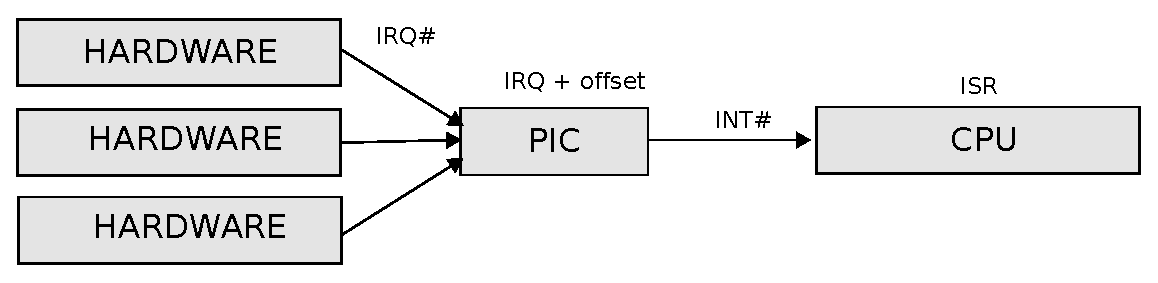
\includegraphics[width=\textwidth]{imgs/drawings/irqs/explanationsvg.eps}
  \caption{Hardware interrupts are translated to software interrupt via the PIC.}
\end{figure}

\par
 Since interrupts keep triggering constantly from various sources, an ISR must choose what should happen if an IRQ is raised while it is still running. There are two options.  The ISR can decide it needs a "long" time to run and disable other IRQs via the IMR\footnote{Interrupt Mask Register}. This path introduces the problem of discarding important information such as keyboard or mouse inputs.\\
 \par
 Alternately, the ISR can decide not to mask other IRQs and do what it is supposed to do as fast as possible so as to not delay the firing of other important interrupts that may lose data if they aren't serviced quickly enough. Keen Dreams uses the latter approach and keeps tasks in its ISR very small and short. 

\subsection{IRQs and ISRs}
The IRQ and ISR system relies on two chips: the Intel 8254, which functions as a Programmable Interval Timer (PIT), and the Intel 8259, which acts as a Programmable Interrupt Controller (PIC). The PIT features a crystal oscillating at 1.193182 MHz. At its core, the PIT is a decrementing counter. The programmer loads a 16-bit value between 0 and 65,535 into a register in the PIT. With each clock pulse, the counter decrements toward zero. Once it reaches zero, it automatically resets to the original value stored in the register and starts over.\\

\par
\begin{figure}[H]
  \centering
  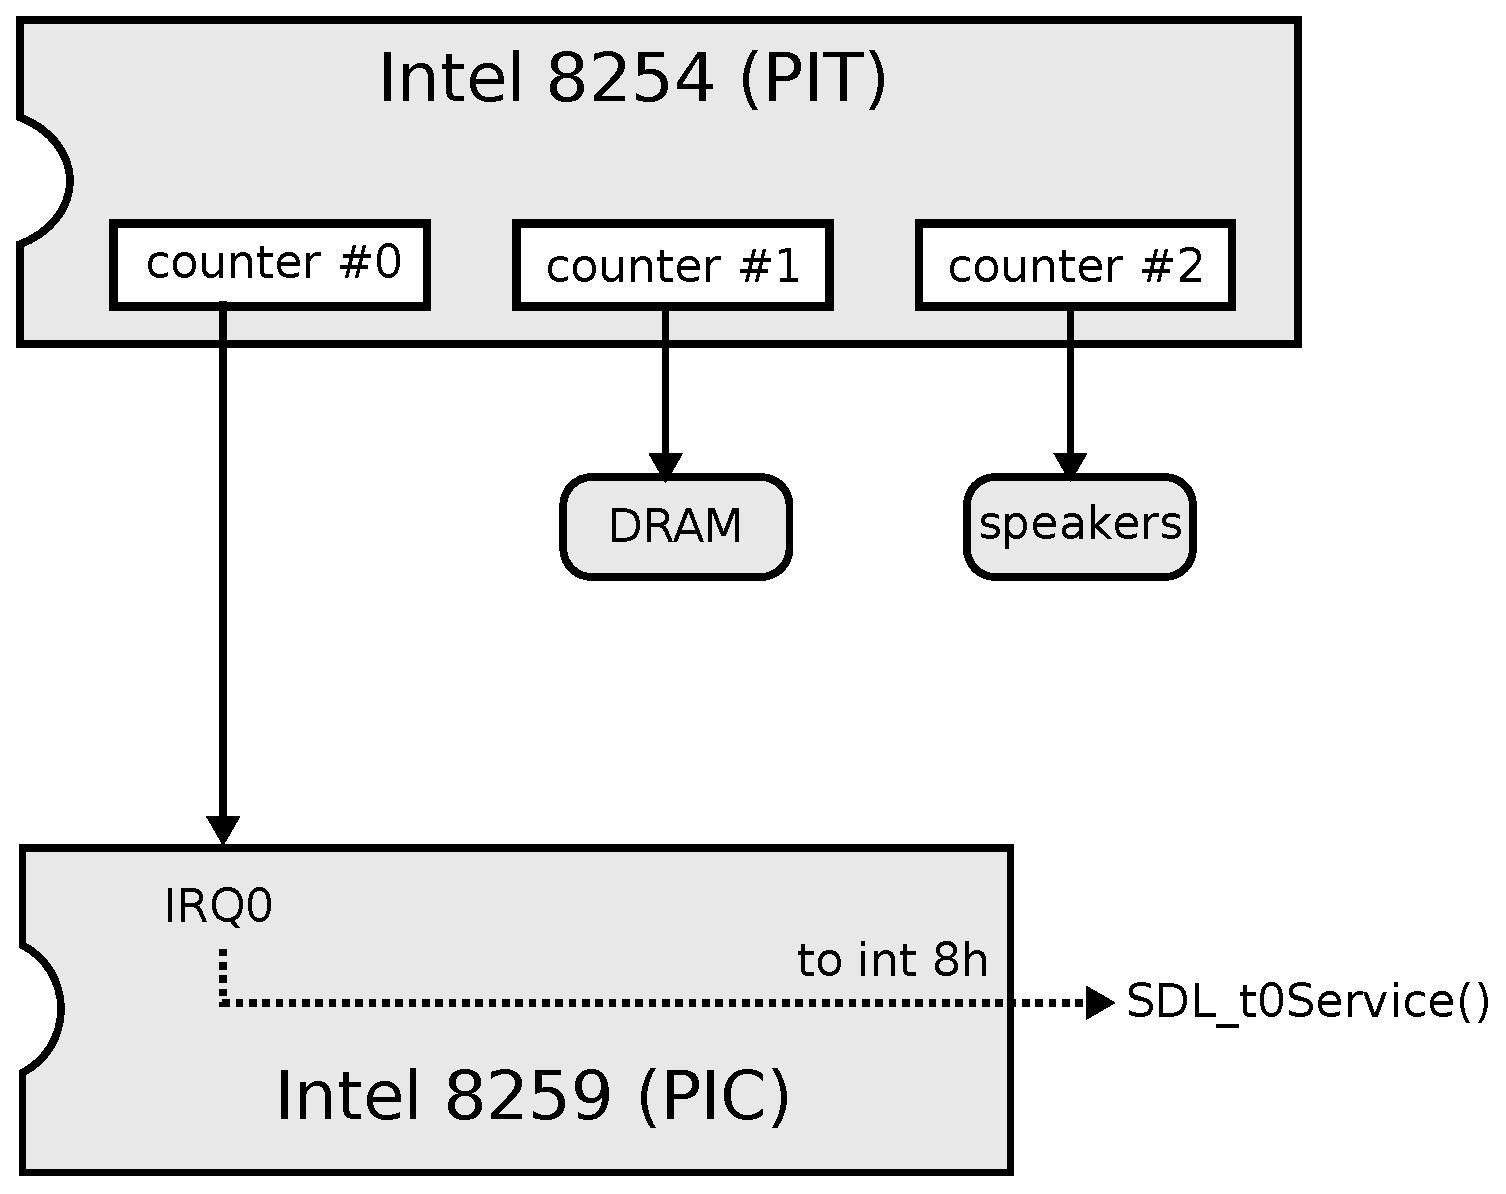
\includegraphics[width=.75\textwidth]{imgs/drawings/heartbeats.eps}
  \caption{Interactions between PIT and PIC.}
\end{figure}

\par
In fact, there are three counters in the PIT. Counter \#1 is connected to the RAM in order to automatically perform something called "memory refresh" and was considered a "do not touch" part of the PIT\footnote{Without frequent refresh, DRAM will lose its content. This is one of the reasons it is slower and SRAM is preferred in the caching system.}. Counter \#2 is connected to the PC speaker and generates sounds, and will be explained in detail in the next section. Counter \#0 is connected to the PIC and when it hits zero it triggers IRQ 0 and sends it to the PIC. The PIC manages hardware interrupts, mapping IRQ 0 - IRQ 8 to the Interrupt Vector Table (IVT), a list of pointers to the corresponding ISR addresses. Notice that IRQ 0 (mapped to IVT entry \#8) is associated with the System timer and usually updates the operating system clock.

\begin{figure}[H]
	\centering
	\begin{tabularx}{\textwidth}{ l p{.5\textwidth}  }
	  \toprule
	  \textbf{IVT Entry \#} & \textbf{Type} \\ \bottomrule

	  00h	&	CPU divide by zero \\
01h	&	Debug single step \\
02h	&	Non Maskable Interrupt \\
03h	&	Debug breakpoints \\
04h	&	Arithmetic overflow \\
05h	&	BIOS provided Print Screen routine \\
06h	&	Invalid opcode \\
07h	&	No math chip \\
08h & IRQ0, System timer \\
09h & IRQ1, Keyboard controller \\
0Ah & IRQ2, Bus cascade services for second 8259 \\
0Bh & IRQ3, Serial port COM2 \\ 
0Ch & IRQ4, Serial port COM1 \\
0Dh & IRQ5, LPT2, Parallel port (HDD on XT) \\
0Eh & IRQ6, Floppy Disk Controller \\
0Fh & IRQ7, LPT1, Parallel port \\
10h & Video services (VGA)\\
11h & Equipment check \\
12h & Memory size determination \\
		\bottomrule
	\end{tabularx}
	\caption{The Interrupt Vector Table (entries 0 to 18).}
\end{figure}

\subsection{Hijacking the System Timer}
By modifying the IVT \#8 pointer, an application can hijack the interrupt to serve its own purposes. When this occurs, the engine halts its runtime at regular intervals and jumps to a custom interrupt function. We now have two systems running in parallel.\\

\par
\begin{minipage}{\textwidth}
\lstinputlisting[language=C,morekeywords={longword}]{code/interrupt_service.c}
\end{minipage}\\

\par
IVT \#8, in its original configuration, not only operates the system clock but also manages the floppy disk motor. Specifically, it ensures the motor shuts off after a read or write operation. When IVT \#8 is hijacked, this functionality is bypassed, causing the floppy disk motor to run indefinitely. Although this does not cause issues, the constant spinning of the disk can be both noisy and confusing, potentially giving users the impression that data loading is still in progress.\\

\par
The current status of the disk motors is stored in the BIOS Data Area (BDA), which is a section of memory located at segment \cw{0040h}. The BDA stores many variables indicating information about the state of the computer.\\

\begin{figure}[H]
	\centering
	\begin{tabularx}{\textwidth}{ l p{.5\textwidth}  }
	  \toprule
	  \textbf{Address \#} & \textbf{Description} \\ \bottomrule
40:00h	&	I/O ports for COM1-COM4 serial \\
40:08h	&	I/O ports for LPT1-LPT3 parallel \\
40:17h	&	Keyboard state flags \\
40:1Eh	&	Keyboard buffer \\
40:3Fh	&	Floppy disk drive motor status \\
40:40h	&	Floppy disk drive motor time-out counter \\
40:41h	&	Floppy disk drive status \\
40:49h & 	Display Mode \\
40:4Ah & 	Number of columns in text mode \\
40:75h & 	Number of hard disk drives detected \\
		\bottomrule
	\end{tabularx}
	\caption{Partial list of BIOS Data Area variables\protect\footnotemark.}
\end{figure}
% \addtocounter{footnote}{0}
  \footnotetext{For a full overview of BIOS Data Area see https://www.stanislavs.org/helppc/bios\_data\_area.html.}
   % \stepcounter{footnote}

\par
BIOS data address \cw{40:3Fh} holds the motor status, where bit 0 indicates if the disk 1 motor is on and bit 1 if the disk 2 motor is on. BIOS data address \cw{40:40h} contains the disk motor shutoff counter. This counter is decremented by the timer interrupt vector. When the counter reaches 0, the disk motor is turned off.\\

\par
The hijacked interrupt subsystem is taking over responsibility for this functionality. It checks whether either disk motor is running and decrements the shutoff counter as needed. When the counter drops below 2, the subsystem invokes the original timer interrupt to ensure the disk motor is properly shut down.\\

\par
\begin{minipage}{\textwidth}
\lstinputlisting[language=C,morekeywords={longword}]{code/disk_motor.c}
\end{minipage}\\
\par

\subsection{Heartbeats}
Each counter on the PIT chip is 16-bit, which is decremented after each period. An IRQ is generated and send to the PIC whenever the counter wraps around after 2$^{16}$ = 65,536 decrements. By default, the interrupts are generated at a frequency of 1.19318MHz / 65,536 = 18.2Hz. To change the interrupt frequency, the timer can be reprogrammed by simply adjusting the counter value.\\

\par
\begin{minipage}{\textwidth}
\lstinputlisting[language=C,morekeywords={longword}]{code/set_timer.c}
\end{minipage}\\
\par

\textbf{\underline{Trivia :}} Note that \cw{SDL\_SetTimer0} is using a frequency of 1.192755MHz, instead of the PIT documented 1.193182MHz. This difference is likely derived from the calculation 18.2 Hz * 65,536 = 1.192755MHz.\\

\par
The engine can decide at what frequency to be interrupted, depending on the type of sound it needs to play and what devices will be used. As a result, two frequencies are defined:
\begin{enumerate}
\item Running at 140Hz to play sound effects and music on the PC beeper, AdLib and SoundBlaster.
\item Running at 700Hz to play sound effects and music on Disney Sound Source.
\end{enumerate}
\par
\begin{minipage}{\textwidth}
\lstinputlisting[language=C]{code/set_sound_mode.c}
\end{minipage}

\par
Each time the interrupt system triggers, it runs another small (yet paramount) system before taking care of audio requests. The sole goal of this heartbeat system is to maintain a 32-bit variable: \cw{TimeCount}.

\par
\begin{minipage}{\textwidth}
\lstinputlisting[language=C,morekeywords={longword}]{code/timecount.c}
\end{minipage}

\par
It is updated at a rate of 70 units per seconds, to match the VGA update rate of 70Hz. These units are called "ticks". Depending on how fast the audio system runs (from 140Hz to 700Hz), it adjusts how frequent it should increase \cw{TimeCount} to keep the game rate at 70Hz.\\

\par
Every system in the engine uses this variable to pace itself. The renderer will not start rendering a frame until at least one tick has passed. The AI system expresses action duration in tick units. The input sampler checks for how long a key was pressed, and the list goes on. Everything interacting with human players uses \cw{TimeCount}.


\subsection{Audio System}
The audio system is complex because of the fragmentation of audio devices it can deal with. The early 90's was a time before Windows 95 harnessed all audio cards under the DirectSound common API. Each development studio had to write their own abstraction layer and id Software was no exception. At a high level, the Sound Manager offers a lean API divided in two categories: one for sounds and one for music.\\

\par
\begin{minipage}{\textwidth}
\lstinputlisting[language=C,morekeywords={longword}]{code/sound1.h}
\end{minipage}
\par
\begin{minipage}{\textwidth}
\lstinputlisting[language=C,morekeywords={longword}]{code/sound.h}
\end{minipage}
\par
\vspace{10pt}

But in the implementation lies a maze of functions directly accessing the I/O port of three sound outputs: AdLib, SoundBlaster and PC Speaker. All belong to one of the two supported families of sound generators: Square Waves (PC speaker) or FM Synthesizer (Frequency Modulation). \\

\par
Sounds effects are stored in two formats.
\begin{enumerate}
\item PC Speaker.
\item AdLib.
\end{enumerate}

They are all packaged in the \cw{AudioT} archive created by Muse. Sounds are segregated by format but always stored in the same order. This way a sound can be accessed in two formats by using \cw{STARTPCSOUNDS} + \cw{sound\_ID} or \cw{STARTADLIBSOUNDS} + \cw{sound\_ID}.\\

\par
Although the Sound Manager was designed to support music and digital sound playback on SoundBlaster and Disney Sound Source, this functionality was never implemented in Keen Dreams (as explained in section \ref{section:audio}) and will be therefore not further explained in this section.\\

\begin{minipage}{\textwidth}
\lstinputlisting[language=C,morekeywords={longword}]{code/muse_header.c}
\end{minipage}



\subsection{PC Speaker}
The hardware chapter described a problem for sound effects: the default PC speaker could only generate square waves, resulting in long beeps which are not acceptable for gaming.\\

\par
Earlier it was hinted that the PIT had three counter channels (0-2), of which channel 2 was used for PC speaker output. The counter output mode can be reprogrammed to "square wave generator" mode. If counter \#2 is closer to its starting value than zero, the output of the PIT is a high electrical signal. If the counter is closer to zero, the output is low. The end result is a square wave, high half of the time and low the other half, with the frequency controlled by the value in the PIT register. This square wave signal is amplified and fed into the speaker. \\

\par
\begin{figure}[H]
  \centering
  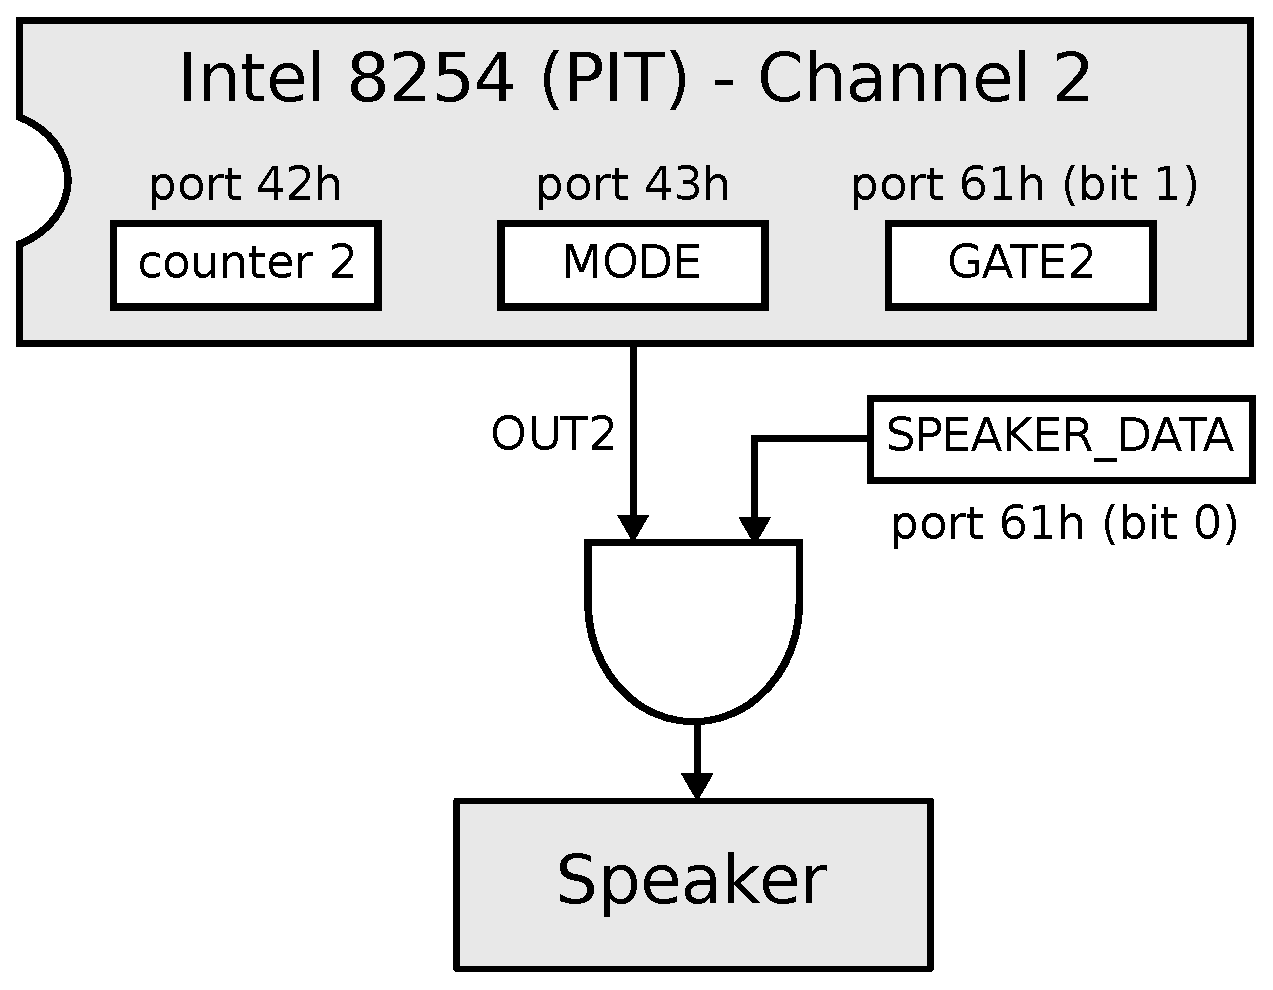
\includegraphics[width=1.0\textwidth]{imgs/drawings/pc_speaker.eps}
  \caption{Built-in speaker hardware diagram.}
  \label{fig:pc_speaker}
\end{figure}

\par
\vspace{10pt}
To adjust the frequency, write to port \cw{43h} to set the PIT command register, followed by writing the desired counter value to port \cw{42h}.\\

\begin{figure}[H]
	\centering
	\renewcommand{\arraystretch}{1.6}
	\begin{tabularx}{\textwidth}{ c c p{.5\textwidth}  }
	  \toprule
	  \textbf{Bit \#} & \textbf{Value} & \textbf{Description} \\ \bottomrule

  0 & 0 & \multirow{2}{*}{Set value for counter 2 (at port \cw{42h}).} \\
  1 & 1 & \\ \hline
  2 & 1 & \multirow{2}{.8\textwidth}{Because the data port is an 8 bit I/O port and the count values is 16 bit, the PIT chip needs to be instructed 16 bits are transferred as a pair, starting with the lowest 8 bits followed by the highest 8 bits.} \\
  3 & 1 & \\ \hline
  4 & 1 & \multirow{3}{*}{Set to square wave generator mode.} \\
  5 & 1 & \\
  6 & 0 & \\ \hline
  7 & 0 & Counter is a 16-bit binary counter (0-65535). \\  
		\bottomrule
	\end{tabularx}
	\caption{Set PIT Command register (port \cw{43h}) to value \cw{b6h}\protect\footnotemark.}
\end{figure}
% \addtocounter{footnote}{0}
  \footnotetext{For details, see https://wiki.osdev.org/Programmable\_Interval\_Timer}
   % \stepcounter{footnote}

\par
The connection to the speaker can be deactivated without changing any timer parameters through the system's keyboard controller (Intel 8042 UPI). Setting port \cw{61h}, bit 0 and bit 1, to 0 turns off both counter \#2 and the speaker.\\

\par
\begin{minipage}{\textwidth}
\lstinputlisting[language=C]{code/pwm_code.c}
\end{minipage}

\par
A simple tone has only one frequency. As a practical example, say we wanted to play a middle C through the speaker. Middle C is 261.626 Hz\footnote{261.626 Hz for middle C is a consequence of the twelve-tone equal temperament, see https://en.wikipedia.org/wiki/12\_equal\_temperament.}, and the PIT clock runs at 1.193182 MHz. Dividing the latter by the former and rounding to the nearest integer value yields 4561. This is the value that must be written to the PIT counter \#2 to produce the desired tone. While the counter is above 2280 the output signal is high, below that threshold the output signal is low. Once the counter reaches 0, it automatically resets to the initial value of 4561 and the cycle repeats. To create a higher pitch, the counter value would need to be lower. \\

\par
<<PICTURE OF WAVES>>\\

\par
When instructed to play a PC Speaker sound effect, the audio system sets itself to run at 140Hz via PIT Counter \#0. Every times it wakes up, it reads the frequency to maintain for the next 1/140th of a second and writes it to Counter \#2.\\

\par
Human hearing ranges from approximately 20 Hz to 20,000 Hz, making any counter value lower than 60 inaudible. Frequencies are encoded in a stream of bytes (0-255) and decoded using the formula\\

\par
\begin{minipage}{\textwidth}
\lstinputlisting[language=C]{code/frequency.c}
\end{minipage}

\par
The lowest frequency is 78 Hz and the highest frequency is 19,886 Hz. Notice how the \cw{* 60} is not calculated but looked up. Once again the engine tries to save as much CPU time as possible by using a bit of RAM. The frequency is read from a lookup table \cw{pcSoundLookup}.\\

\par
\begin{minipage}{\textwidth}
\lstinputlisting[language=C,morekeywords=word]{code/pcSoundLookup.c}
\end{minipage}
\par

\subsection{AdLib}
The AdLib sound relies on the OPL2 chip. Programming the OPL2 output is esoteric to say the least. AdLib and Creative did publish SDKs but they were expensive.  Documentation was sparse and often cryptic. Today, they are very difficult to find.\\
\par
The OPL2 is made of 9 channels capable of emulating instruments. Each channel is made of two oscillators: a Modulator whose outputs are fed into a Carrier's input. Each channel has individual settings including frequency and envelope (composed of attack rate, decay rate, sustain level, release rate, and vibrato). Each oscillator can also pick a waveform (these characteristic forms are what gave the YM3812 its recognizable sound).\\
\par
 To control all of these channels, a developer must configure the OPL2's 244 internal registers. These are all accessed via two external I/O ports. One port is for selecting the card's internal register and the other is to read/write data to it.\\
\par
\begin{minipage}{\textwidth}
\lstinputlisting[language=C,morekeywords={longword}]{code/audio_ports.c}
\end{minipage}
\par
When the AdLib was first conceived in 1986, it was tested on IBM XTs and ATs, none of which exceeded a speed of 6 MHz. They wrote their specification based on this, writing that while the AdLib required a certain amount of "wait time" between commands, it was okay to send them as fast as possible because no PC was faster than the minimum wait time. They later found out that a Intel 386 was fast enough to send commands faster than the AdLib was expecting them, and they changed their specification to mention a minimum 35 microseconds wait time between commands.\\

\par
The Programming Guide was amended with reliable specs to wait 3.3 microseconds after a register select write, and 23 microseconds after a data write. For Keen Dreams it is implemented as a 10 microseconds and 25 microseconds respectively.
\par
\begin{minipage}{\textwidth}
\lstinputlisting[language=C,morekeywords={longword}]{code/adlib_wait.c}
\end{minipage}
\par

The engine does not know about any of the details of the OPL2. There is zero abstraction layer of transformation here. An IMF sound is made of a series of messages containing the values to write to the register and data ports of the OPL2.\\

\par
Every time the audio system wakes up via the timer interrupt, it checks if a sound effects should be sent, and plays the next sample out through the AdLib card.\\



\end{document}










